\documentclass[../../main.tex]{subfiles}
\begin{document}

{\bf [解答]}

\begin{figure}[htb]
  \centering
  \begin{tikzpicture}[scale=1.5, >=stealth, every node/.style={font=\small}]
    \coordinate (O) at (0, 0);
    \draw[->, thick, gray!80!black] (-1.3, 0) -- (3.0, 0) node[right] {$x$};
    \draw[->, thick, gray!80!black] (0, -1.3) -- (0, 2.5) node[above] {$y$};
    \node[below left=2pt] at (O) {$O$};

    % 単位円
    \draw[line width=1.1pt, blue!75!black] (O) circle (1);
    \node[below right] at (1, 0) {$1$};

    % x = a の直線
    \draw[dashed, gray!60] (2.2, -0.5) -- (2.2, 2.4);
    \node[below] at (2.2, 0) {$a$};
    \node[above, gray!70!black] at (2.2, 2.4) {$x=a$};

    % 時刻 t での一直線状態 (例として角 45 度)
    \coordinate (P) at (45:1);
    \coordinate (Q) at (2.2, 2.2);

    % 直線 OPQ
    \draw[orange!85!black, thick] (O) -- ($(O)!1.15!(Q)$);

    % 動点 P, Q
    \node[circle, fill=blue!85!black, inner sep=1.5pt] at (P) {};
    \node[circle, fill=red!85!black, inner sep=1.5pt] at (Q) {};
    \node[above left] at (P) {$P_t(\cos\pi t, \sin\pi t)$};
    \node[right=2pt] at (Q) {$Q_t(a, vt)$};

    % 速度矢印
    \draw[->, thick, red!85!black] (Q) -- ++(0, 0.5) node[right] {$v$};
    \draw[->, thick, blue!85!black] (P) -- ++(-0.35, 0.35) node[above left=-1pt] {$\pi$};

    % 角度マーク
    \draw[gray!70] (0.4, 0) arc (0:45:0.4);
    \node[font=\footnotesize] at (22.5:0.55) {$\pi t$};
  \end{tikzpicture}
  \caption{動点 $P_t$ と $Q_t$ の配置，および $O,P,Q$ が一直線上に並ぶ様子．}
  \label{fig:1971_6_points_motion}
\end{figure}

時刻 $t$ の $P, Q$ の座標は
\begin{align}
  P_t (\cos \pi t, \sin \pi t), \quad Q_t (a, vt) \quad (0 < v < a\pi) \label{eq:1}
\end{align}
である.

\paragraph{(1)}

$O,P,Q$が一直線上に並ぶのは，$\overrightarrow{OP_t} \parallel \overrightarrow{O Q_t}$と同値であるからこうなる条件を調べる．\cref{eq:1}より
\begin{align}
  \overrightarrow{OP_t} \parallel \overrightarrow{O Q_t}
  \iff
  v t \cos \pi t - a \sin \pi t = 0 \label{eq:2}
\end{align}
である．この左辺を $f(t)$ とおく：
\begin{align}
  f(t) = v t \cos \pi t - a \sin \pi t \label{eq:3}
\end{align}
と，一階微分は
\begin{align}
  f'(t)
  & = v \cos \pi t - \pi v t \sin \pi t - \pi a \cos \pi t \\
  & = -(\pi a - v) \cos \pi t - \pi v t \sin \pi t \label{eq:4}
\end{align}
である. 三角関数の合成から
\begin{align}
  f'(t) = -\sqrt{(\pi a - v)^2 + (\pi v t)^2} \sin(\pi t + \alpha) \label{eq:5}
\end{align}
とおける. ただし $\alpha$ は
\begin{align}
  \cos \alpha = \dfrac{\pi v t}{\sqrt{(\pi a - v)^2 + (\pi v t)^2}}, \quad
  \sin \alpha = \dfrac{\pi a - v}{\sqrt{(\pi a - v)^2 + (\pi v t)^2}} \label{eq:6}
\end{align}
を満たす $0 < \alpha < \dfrac{\pi}{2}$ なる角である．

従って$n < t \le n+1$ の時,
\begin{align}
  n\pi + \alpha \le \pi t + \alpha \le (n+1)\pi + \alpha
\end{align}
となり, $f'(t)$ は区間内で符号をかえる点$t=t'$をただ一つ
\begin{align}
  \pi t' + \alpha = (n+1)\pi
  \quad \therefore
  t' = n+1 - \dfrac{\alpha}{\pi} \label{eq:7}
\end{align}
に持つ．よって$n$の偶奇に応じて増減表は以下のようになる．

\begin{table}[htb]
  \centering
  \caption{$n=2k$の時の$f(t)$の増減表}
  \begin{tabular}{c|c|c|c|c|c}
    $t$ & $2k$ & $\dots$ & $t'$ & $\dots$ & $2k+1$ \\ \hline
    $f'$ & & $-$ & $0$ & $+$ & \\ \hline
    $f$ & 正 & $\searrow$ & & $\nearrow$ & 負
  \end{tabular}
\end{table}

\begin{table}[htb]
  \centering
  \caption{$n=2k+1$の時の$f(t)$の増減表}
  \begin{tabular}{c|c|c|c|c|c}
    $t$ & $2k+1$ & $\dots$ & $t'$ & $\dots$ & $2k+2$ \\ \hline
    $f'$ & & $+$ & $0$ & $-$ & \\ \hline
    $f$ & 負 & $\nearrow$ & & $\searrow$ & 正
  \end{tabular}
\end{table}

\begin{figure}[htb]
  \centering
  \begin{tikzpicture}[scale=1.1, >=stealth, every node/.style={font=\small}]
    % --------------------------------------------------------
    % n = 2k
    % --------------------------------------------------------
    \begin{scope}[shift={(0, 0)}]
      \draw[->, thick, gray!80!black] (-0.3, 0) -- (4.2, 0) node[right] {$t$};
      \draw[->, thick, gray!80!black] (0, -1.8) -- (0, 1.8) node[above] {$f(t)$};

      \coordinate (T0) at (0.5, 0);
      \coordinate (T1) at (3.5, 0);
      \coordinate (Tn) at (1.4514, 0);
      \coordinate (Tp) at (3.1277, 0);
      \coordinate (Mp) at (3.1277, -1.292);

      % 曲線: f(t) = (2+u)*cos(pi*u) - 1.5*sin(pi*u) をスケーリング
      \draw[line width=1.3pt, blue!85!black, domain=0.5:3.5, samples=60]
      plot (\x, { ((2 + (\x-0.5)/3.0)*cos(180*(\x-0.5)/3.0) - 1.5*sin(180*(\x-0.5)/3.0)) / 2.5 });

      \node[below] at (T0) {$2k$};
      \node[below] at (T1) {$2k+1$};

      % 零点 t_n
      \node[circle, fill=red!85!black, inner sep=1.4pt] at (Tn) {};
      \node[below=2pt, red!85!black] at (Tn) {$t_n$};

      % 極小点 t'
      \draw[dashed, gray!60] (Tp) -- (Mp);
      \node[circle, fill=gray!70!black, inner sep=1.2pt] at (Mp) {};
      \node[above=2pt] at (Tp) {$t'$};

      \node[below=16pt] at (2.0, 0) {$n=2k$ のとき};
    \end{scope}

    % --------------------------------------------------------
    % n = 2k + 1
    % --------------------------------------------------------
    \begin{scope}[shift={(5.2, 0)}]
      \draw[->, thick, gray!80!black] (-0.3, 0) -- (4.2, 0) node[right] {$t$};
      \draw[->, thick, gray!80!black] (0, -1.8) -- (0, 1.8) node[above] {$f(t)$};

      \coordinate (T0b) at (0.5, 0);
      \coordinate (T1b) at (3.5, 0);
      \coordinate (Tnb) at (1.5997, 0);
      \coordinate (Tpb) at (3.2195, 0);
      \coordinate (Mpb) at (3.2195, 1.304);

      % 曲線: f(t) = -(3+u)*cos(pi*u) + 1.5*sin(pi*u) をスケーリング
      \draw[line width=1.3pt, blue!85!black, domain=0.5:3.5, samples=60]
      plot (\x, { (-(3 + (\x-0.5)/3.0)*cos(180*(\x-0.5)/3.0) + 1.5*sin(180*(\x-0.5)/3.0)) / 3.2 });

      \node[below] at (T0b) {$2k+1$};
      \node[below] at (T1b) {$2k+2$};

      % 零点 t_n
      \node[circle, fill=red!85!black, inner sep=1.4pt] at (Tnb) {};
      \node[below=2pt, red!85!black] at (Tnb) {$t_n$};

      % 極大点 t'
      \draw[dashed, gray!60] (Tpb) -- (Mpb);
      \node[circle, fill=gray!70!black, inner sep=1.2pt] at (Mpb) {};
      \node[below=2pt] at (Tpb) {$t'$};

      \node[below=16pt] at (2.0, 0) {$n=2k+1$ のとき};
    \end{scope}
  \end{tikzpicture}
  \caption{区間 $[n,n+1]$ における $f(t)$ の概形と，唯一の零点 $t_n$．}
  \label{fig:1971_6_f_curves}
\end{figure}

従って, $n \le t_n \le n+1$ の間に $f(t_n) = 0$ をみたす $t_n$ が唯一ある.

\paragraph{(2)}

題意より$n \le t_n \le n+1$であり，$f(t_n)=0$が成り立つ．
\cref{eq:3}に$t=t_n$を代入して
\begin{align}
  & v t_n \cos \pi t_n - a \sin \pi t_n = 0 \\
  \therefore
  & \cos \pi t_n = \dfrac{a \sin \pi t_n}{v t_n} \xrightarrow{n\to\infty} 0 (\because t_n \to \infty) \\
  \therefore
  & \lim_{n\to\infty} \cos \pi (t_n-n) = 0 \quad (0 \le t_n-n \le 1)
\end{align}
である．従ってこれを満たす$t_n-n$を考えて
\begin{align}
  \lim_{n\to\infty}t_n - n = \dfrac{1}{2}
\end{align}
であり，$t_n-n$は一定値$\dfrac{1}{2}$に近づく．

{\bf [別解]}

\paragraph{(1)}

\begin{figure}[htb]
  \centering
  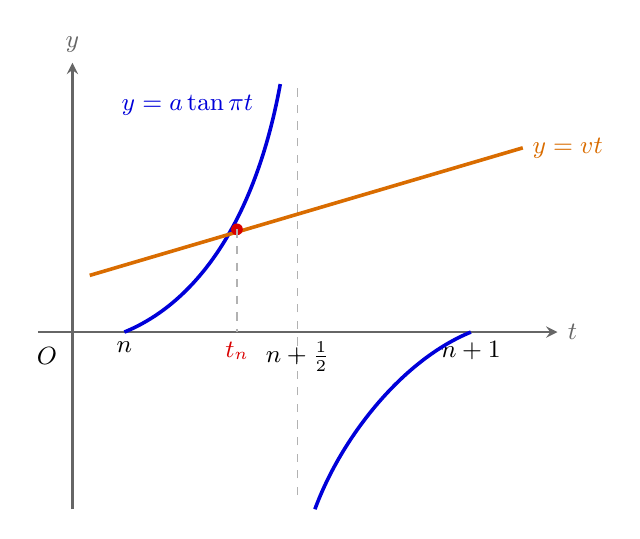
\begin{tikzpicture}[x=2.2cm, y=0.9cm, >=stealth, every node/.style={font=\small}]
    \draw[->, thick, gray!80!black] (-0.2, 0) -- (2.8, 0) node[right] {$t$};
    \draw[->, thick, gray!80!black] (0, -2.5) -- (0, 3.8) node[above] {$y$};

    \coordinate (N) at (0.3, 0);
    \coordinate (Asymp) at (1.3, 0);
    \coordinate (N1) at (2.3, 0);

    % 漸近線 t = n + 1/2
    \draw[dashed, gray!60] (1.3, -2.3) -- (1.3, 3.5);
    \node[below] at (N) {$n$};
    \node[below] at (Asymp) {$n+\frac{1}{2}$};
    \node[below] at (N1) {$n+1$};

    % y = a tan(pi t)
    \draw[line width=1.3pt, blue!85!black]
    (0.3, 0) .. controls (0.7, 0.4) and (1.05, 1.5) .. (1.2, 3.5);
    \draw[line width=1.3pt, blue!85!black]
    (1.4, -2.5) .. controls (1.55, -1.5) and (1.9, -0.4) .. (2.3, 0);
    \node[blue!85!black, left] at (1.1, 3.2) {$y=a\tan\pi t$};

    % y = vt
    \draw[line width=1.3pt, orange!85!black] (0.1, 0.8) -- (2.6, 2.6);
    \node[orange!85!black, right] at (2.6, 2.6) {$y=vt$};

    % 交点 t_n
    \coordinate (Inters) at (0.95, 1.45);
    \node[circle, fill=red!85!black, inner sep=1.5pt] at (Inters) {};
    \draw[dashed, gray!60] (Inters) -- (0.95, 0);
    \node[below, red!85!black] at (0.95, 0) {$t_n$};

    \node[below left=2pt] at (0, 0) {$O$};
  \end{tikzpicture}
  \caption{$y=a\tan\pi t$ と $y=vt$ のグラフの交点 $t_n$．}
  \label{fig:1971_6_tan_intersection}
\end{figure}

\cref{eq:2}より$t \neq n+\dfrac{1}{2}$だから両辺を$\cos \pi t$で割って
\begin{align}
  vt = a\tan \pi t
\end{align}
である．これは確かに$[n,n+1]$でただ一つの解を持つ．

\end{document}
